\chapter*{Introduction}

Diese Masterarbeit befasst sich mit der Problemstellung der Generierung von Roboterplänen im Kontext von Mixing Aktionen, welche aus einer Wissensbasis abgeleitet werden.
Bevor wir mit der Vorstellung der Gliederung der Masterarbeit anfangen, möchten wir auf 5 essenzielle Fragen eingehen, um den Lesern einen besseren Überblick geben zu können:
\begin{itemize}
    \item \textbf{Was ist das Problem?} In der Welt des Kochen und Backen müssen verschiedene Tätigkeiten ausgeführt werden. Während ein Mensch im Laufe seines Lebens erlernt, wie Rezepte zubereitet werden und intuitiv die benötigten Aktionen ausführt, muss ein Roboter die benötigten Aktionen abrufbar haben. Die Aufgaben eines Roboters im Kontext vom Kochen können vielfältig sein, wie zum Beispiel das Schneiden, Gießen oder Rühren. In dieser Arbeit befassen wir uns mit der Aufgabe des Rührens und betrachten dabei das Problem der verschiedenen Rühraktionen und in welchem Zusammenhang diese ausgeführt werden. 
    \item \textbf{Warum ist es wichtig?} Im Kontext des Mixen müssen verschiedene Bewegungen betrachtet werden um die gewünschten Resultate zu erzielen. Es reicht nicht eine einzelne Bewegung als Pauschalbewegung im Kontext des Mixings zu betrachten, da sonst verschiedene Ausgänge einer Mixingaktion nicht erreicht werden können. Deshalb muss man verschiedene Bewegungen in Betracht ziehen um gewünschte Resultate einer Mixingaktion erzielen zu können.
    \item \textbf{Warum ist es schwierig?} Die Schwierigkeit liegt darin zu bestimmen unter welchen Umständen welche Bewegung ausgeführt wird. Dies erfordert eine genauere Analyse bestehender Quellen woraus die verschiedenen Bewegungen extrahiert werden können. Eine weitere Herausforderung liegt darin dieses Wissen dementsprechend zu repräsentieren.
    \item \textbf{Wie wird das Problem gelöst?} Um dieses Problem zu lösen implementieren wir eine Wissensbasis, woraus ein Roboteragent die benötigte Bewegung samt Parameter ableiten kann. Die Bewegung leitet sich ab aus der angegeben Aufgabe und aus der Menge der genutzten Zutaten.
    \item \textbf{Wie kann diese Arbeit zur Forschung beitragen?} Durch die Implementierung unserer Wissenbasis ist es dementsprechend möglich für Roboteragenten das benötigte Wissen für die Mixingaktionen abzufragen. Unser Beitrag richtet sich an die Entwicklung von Robotern, welche im Haushalt tätig sind und autonom nicht-triviale Aufgaben ausführen können ohne eine festgelegte Umgebung zu haben.
\end{itemize}


First, we intend to analyze existing research, particularly examining studies that delve into diverse mixing motions and exploring related systems that contain a queryable knowledge graph.
In the following section, we will introduce the reader with the frameworks employed to accomplish our objectives.	
Subsequently, we will present our approach to data acquisition and data representation.
In this chapter, we aim to explain the mixing tasks under consideration and articulate our methodology for representing this data to enable effective querying.
In the subsequent section, we will illustrate the implementation of our rules, with the ultimate aim of determining the appropriate motion to be employed.
To validate our concept, we have opted to simulate various scenarios and assess their outcomes, demonstrating the efficacy of our implemented system.
Finally, we will delve into the discussion of our results and draw conclusions to wrap up our work.

The following graphic is intended to provide an overview and will be referenced in each chapter to indicate which part of the work the chapter is addressing.
\begin{figure}[H]
    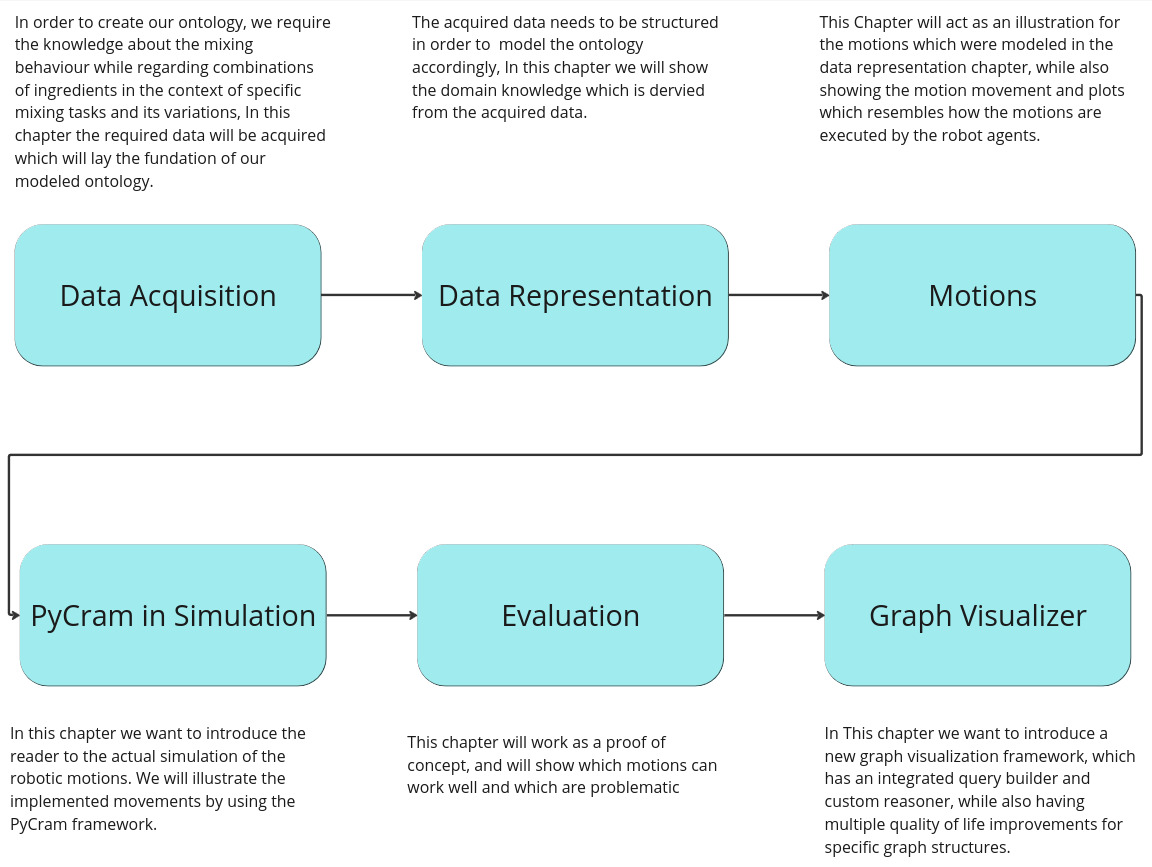
\includegraphics[scale=0.36]{Graphics/overview.jpg}
\end{figure}